\begin{section}{The original result}
The last two theorems of the previous chapter give us enough power to achieve our goal - asymptotic restriction of the worst case chain length. Once again we achieve this limit when hashing even super-linear amount of $n \log n$ elements into $n$ slots. By hashing a linear amounts this expected length can not grow. Every hashed set can be extended into $n \log n$ elements and the estimate must still remain valid. 

The most common models use load factors lower than one. Because of these models we generalise theorem so that it is parametrised by the table's load factor. Important relation of the expected length of the longest chain on the table's load factor is found. The result is that the multiplicative constant of the asymptotic growth is relative to the load factor of a hash table. New results are achieved by modifications of the given proofs with some new ideas.

\begin{theorem}
\label{theorem-n-logn-to-n}
Let $U = \vecspace{w}$ be the hashed universe, $B = \vecspace{t}$ be the hash table and $S \subset U$ be the hashed set such that $|S| = m \log m$ where $t \in \mathbb{N}, m = 2 ^ t$. Let $H = LT(\vecspace{w}, \vecspace{t})$ be the universal system used. Then 
\[
	\Expect{\lpsl} \in O(\log m \log \log m) \text{.}
\]
\end{theorem}
The original proof is showed in the following few pages. It contains some remarks and definitions that are pointed out on their own and later refined. It uses two basic ideas; factorisation and probability estimates of two correlated events.

Let the target space, representation of the hash table, be denoted by $B = \vecspace{t}$. As in the previous proof we will factor a linear transformation $T \in H$, $T: \vecspace{w} \rightarrow \vecspace{t}$. We define factor vector space $A = \vecspace{u}$ for $u \geq \log n$ and two functions $T_0: \vecspace{w} \rightarrow \vecspace{u}$ and $T_1: \vecspace{u} \rightarrow \vecspace{t}$ which is surjective. Both linear functions $T_0$ and $T_1$ are selected uniformly among $LT(U, A)$ and $LTS(A, B)$ respectively. By direct use of model \ref{remark-model-uniform-linear-map-selection} we obtain uniform choice of the transformation $T = T_1 \circ T_0$ .

The second idea of the proof is to estimate the probability of event called $E1$, $\lpsl > l$, for any natural number $l$. The probability bound on $E_1$ is found by inspecting another quite unnatural event $E_2$. Probability of event $E_1$ is then simply determined by discovering the probabilities $\Prob{E_2 | E_1}$ and $\Prob{E_2}$.

\begin{definition}
Let $l$ be a natural number, $T: U \rightarrow B$ be a linear transformation and $S \subset U$ be the hashed set. Event $E_1(S, T, l)$ denotes existence of a chain of length at least $l$ elements when using function $T$. 
\[ 
	E_1(S, T, l) \equiv \exists \vec{y} \in B: | T^{-1}(\vec{y}) \cap S | > l
\]
\end{definition}

\begin{definition}
Let $T_0: U \rightarrow A, T_1: A \rightarrow B$ be linear transformations where $T_2$ is surjective and $S \subset U$ be the hashed set. Event $E_2(S, T_0, T_1)$ is then defined as:
\[
	E_2(S, T_0, T_1) \equiv \exists \vec{y} \in B: T_1^{-1}(\vec{y}) \subseteq T_0(S) \text{.}
\]
\end{definition}

When it is clear what we mean by $S, T_0, T_1$ and $t$ we omit the parametrisation of the events and just use $E_1$ or $E_2$.

Now we will point out another definition of the event $E_2$ that fits better to the scheme of remark $\ref{theorem-linear-function-set-onto}$.
\begin{remark}
\label{remark-e2-equivalency}
Let $T_0: U \rightarrow A$ and $T_1: A \rightarrow B$ be linear transformations and moreover $T_2$ be surjective. Let $S \subset U$ be the hashed set. Appearance of event $E_2(S, T_0, T_1)$ is then equivalent to
\[
	E_2(S, T_0, T_1) \equiv \exists \vec{y}: T_1^{-1}(\vec{y}) \subseteq T_0(S) \Leftrightarrow T_1(A - T_0(S)) \neq B \text{.}
\]
\end{remark}
\begin{proof}
To proof direction from the left to the right assume that event $E_2$ is present. Event $E_2$ occurs if and only if there is a vector $\vec{y} \in B$ such that $T_1^{-1}(\vec{y}) \subseteq T_1(S)$. Under these conditions transformation $T_1$ may not display set $A - T_0(S)$ onto $B$ since $\vec{y} \notin T_1(A - T^{-1}(y)) \supseteq T_1(A - T_0(S))$ or equivalently $B \neq T_1(A - T_0(S))$.

If $B \neq T_1(A - T_0(S))$ then there exists a vector $\vec{y} \in B$ such that $\vec{y} \notin T_1(A - T_0(S))$. Since $T_1$ is surjective we have $T_1(A) = B$. Because no point from $A - T_0(S)$ is displayed on $\vec{y}$ the whole preimage of $\vec{y}$ must be contained in $T_0(S)$, $T_1^{-1}(\vec{y}) \subseteq T_0(S)$.

\begin{figure}
  \centering
    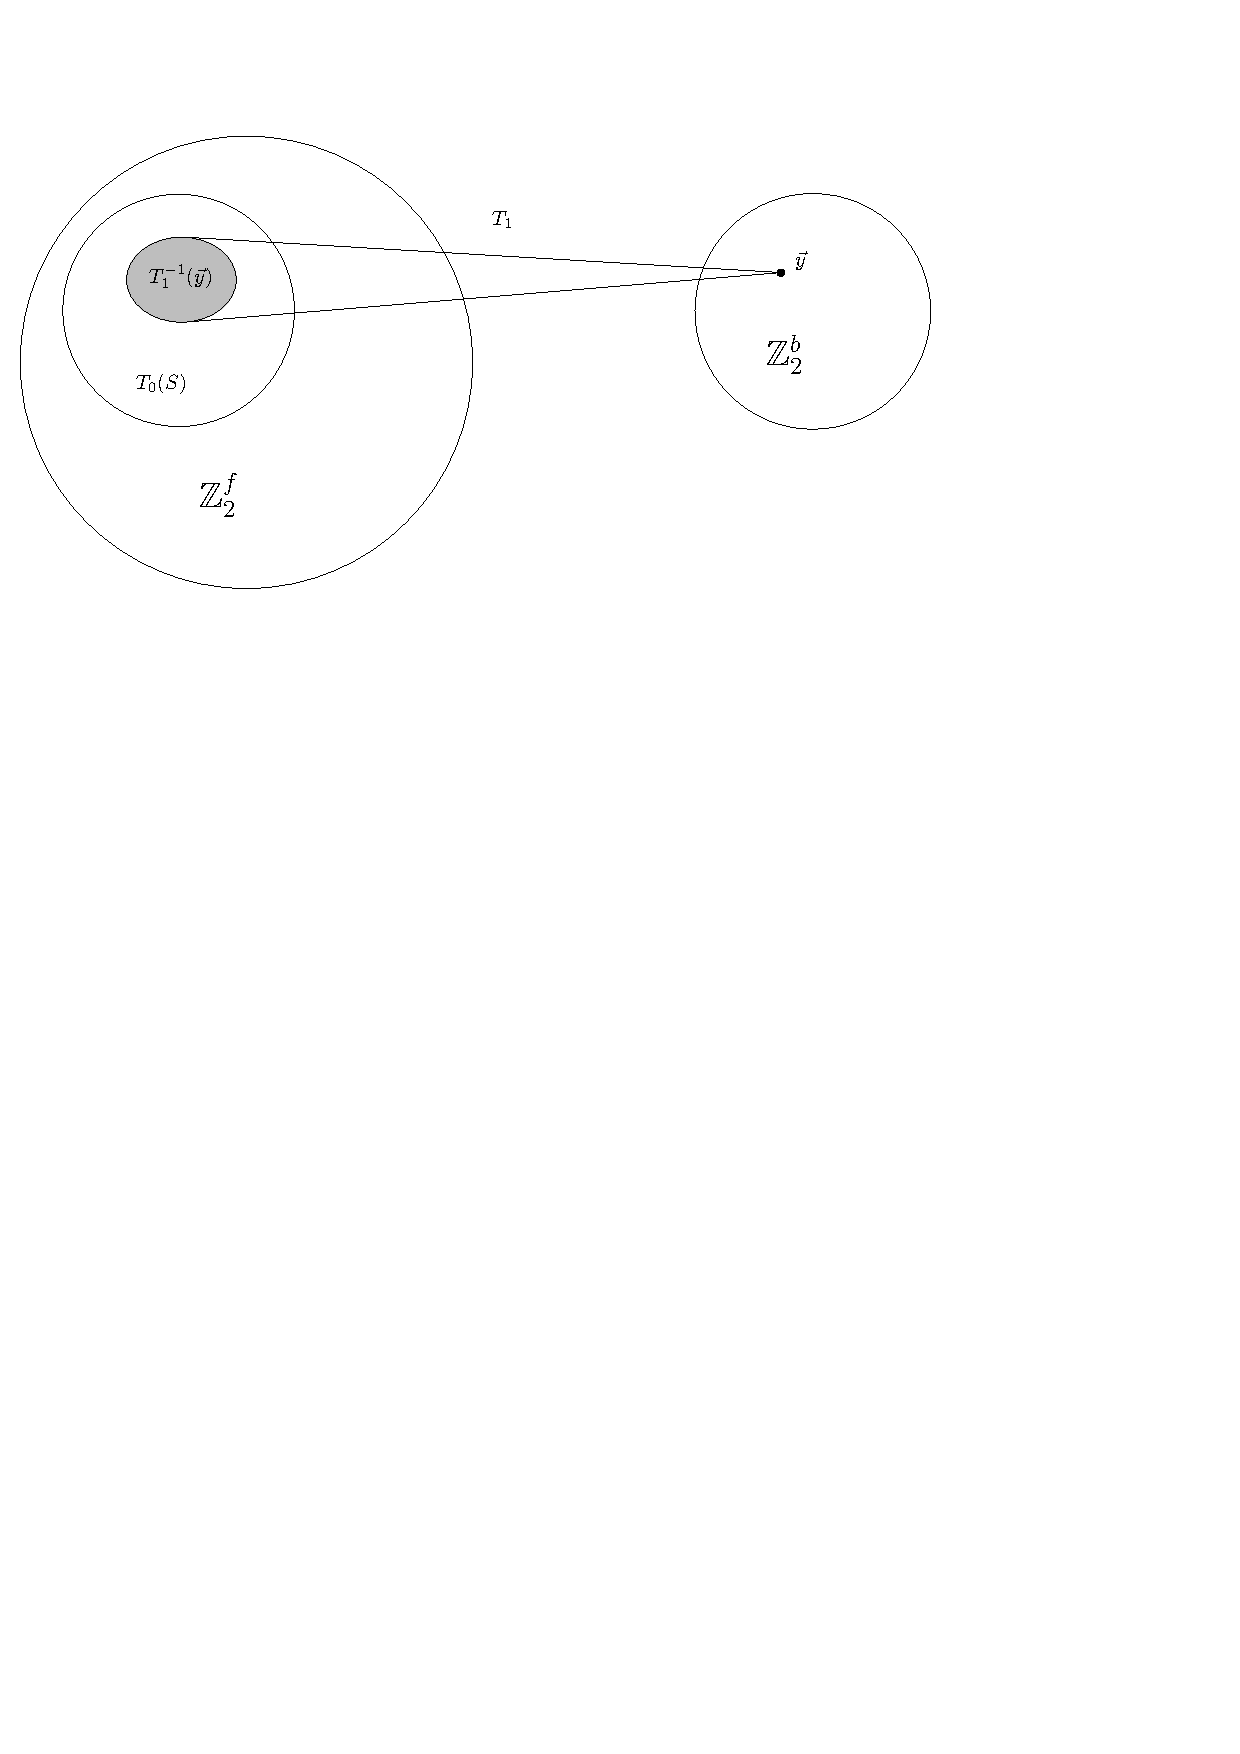
\includegraphics[width=0.7\textwidth]{images/e2}

  \caption{Occurrence of the event $E_2$.}
\end{figure}

\end{proof}

As mentioned before we can use the previous equivalency to estimate probability of event $E_2$ as stated in the following remark. 
\begin{remark}
\label{remark-e2-probability}
Let $U = \vecspace{w}$, $A = \vecspace{u}$ and $B = \vecspace{t}$. Let $T_0: U \rightarrow A$ and $T_1: A \rightarrow B$ be linear transformations where $T_1$ is surjective and $S \subset U$ denote the hashed set such that $|S| \leq |B| \log |B|$. Define $d = \frac{|A|}{|S|}$. If $d > 1$ then 
\[
	\Prob{E_2(S, T_0, T_1))} \leq d^{-\log d - \log \log d} \text{.}
\]
\end{remark}
\begin{proof}
Theorem \ref{theorem-linear-function-set-onto} for surjective transformation $T_1$, set $A - T_0(S) \subset A$, target space $B = \vecspace{t}$ and $\mu = \frac{|T_0(S)|}{|A|}$ states that
\[
	\Prob{T_1(A - T_0(S)) \neq B} \leq \mu ^ {u - t - \log t + \log \log \frac{1}{\mu}} \text{.}
\]

Corresponding inverse density $\mu$ can be computed as 
\[
	\mu = 1 - \frac{|A - T_0(S)|}{|A|} = 1 - \frac{|A| - |T_0(S)|}{|A|} = \frac{|T_0(S)|}{|A|} \leq \frac{|S|}{|A|} = \frac{1}{d} < 1 \text{.}
\] 

Now we can rewrite logarithm of variable $d$ as 
\[
	\log d = \log \frac{|A|}{|S|} = \log |A| - \log |S| \geq \log |A| - \log (|B| \log |B|) = u - t - \log t \text{.}
\]

Since $E_2 \equiv T_1(A - T_0(S)) \neq B$ we can conclude
\[
\begin{split}
\Prob{E_2}
	& \leq \mu^{u - t - \log t + \log \log \left(\frac{1}{\mu}\right)} \\
	& \leq \mu ^ {\log d + \log \log \left(\frac{1}{\mu}\right)} \\
	& \leq \left(\frac{1}{d}\right) ^ {\log d + \log \log d} \\
	& = d ^ {-\log d - \log \log d} \text{.} \\
\end{split}
\]

Because of the assumptions of theorem \ref{theorem-linear-function-set-onto} the proof of this remark holds only when $\emptyset \neq A - T_0(S) \neq A$. Since $S$ is non-empty set we can see that $A - T_0(S) \neq A$. Because $d = \frac{|A|}{|S|} > 1$ it must be true that $|A| > |S| \geq |T_0(S)|$ and set $A - T_0(S)$ can not be empty.
\end{proof}

A similar lemma for estimating the conditional probability of event $E_2 | E_1$ follows.
\begin{remark}
\label{remark-prob-l-length-chain}
Let $U = \vecspace{w}$, $A = \vecspace{u}$ and $B = \vecspace{t}$. Let $T_0: U \rightarrow A$ and $T_1: A \rightarrow B$ be random uniformly chosen linear transformations where $T_1$ is surjective. Then for every $0 < \epsilon < 1$ there is a constant $c_{\epsilon} > 0$ such that for every $S \subset U$ denoting the hashed  elements and for every $l \in \mathbb{N}$, $l \geq c_{\epsilon}{\frac{|A|}{|B|}}\log\frac{|A|}{|B|}$ the upper bound for the probability of event $E_2 | E_1$ is
\[
	\Prob{E_2(S, T_0, T_1) | E_1(S, T, l)} \geq 1 - \epsilon \text{.}
\]
\end{remark}
\begin{proof}
Suppose that we are given a mapping $T$ and the event $E_1$ appears. There must be a subset $S' \subseteq S$ consisting of at least $l$ elements mapped by $T$ to a single element $\vec{y} \in B$. We fix this element and define $U' = T^{-1}(\vec{y})$ and $A' = T_1^{-1}(\vec{y})$. Notice that $S' = U' \cap S$.

From lemma \ref{lemma-linear-transformation-domain-distribution} it follows that size of the set $A'$ is exactly $\frac{|A|}{|B|}$. And from lemma \ref{lemma-linear-transformation-domain-distribution} we have that sets $A'$ and $U'$ are affine subspaces. Since $T_0$ is random uniformly chosen linear mapping its restriction $T_0|_{U'}$ is also a random and uniformly chosen linear transformation as stated in model \ref{remark-model-uniform-linear-map-selection-affine}.

Since we assumed presence of $E_1$ cardinality of $S' = U' \cap S$ must be at least $l \geq c_{\epsilon}\frac{|A|}{|B|} \log\frac{|A|}{|B|} = c_{\epsilon}{A'}\log{A'}$. Now we can use theorem \ref{theorem-set-onto-by-linear-transform} for the source space $U'$, set $S' \subseteq U'$, target space $A'$ and mapping $T_0|_{U'}$ and we obtain that 
\[
	\Prob{T_0|_{U'}(S') = A' | E_1} \geq 1 - \epsilon \text{.}
\]

Remark that we used theorem \ref{theorem-set-onto-by-linear-transform} for affine mapping $T_0|_{U'}$. However, we can use the generating mapping of $T_0|_{U'}$, corresponding non-affine subspaces and transform $S'$ to the original non-affine subspace instead.

Event $E_2$ is certainly present whenever $A' \subseteq T_0(S)$. In the language of probability:
\[
	\Prob{A' \subseteq T_0(S) | E_1} \leq \Prob{E_2 | E_1} \text{.}
\]

Finally we can finish the remark's proof
\[
	\Prob{E_2 | E_1} \geq \Prob{A' \subseteq T_0(S) | E_1} \geq \Prob{A' = T_0|_{U'}(S') | E_1} \geq 1 - \epsilon \text{.}
\]

\begin{figure}
  \centering
    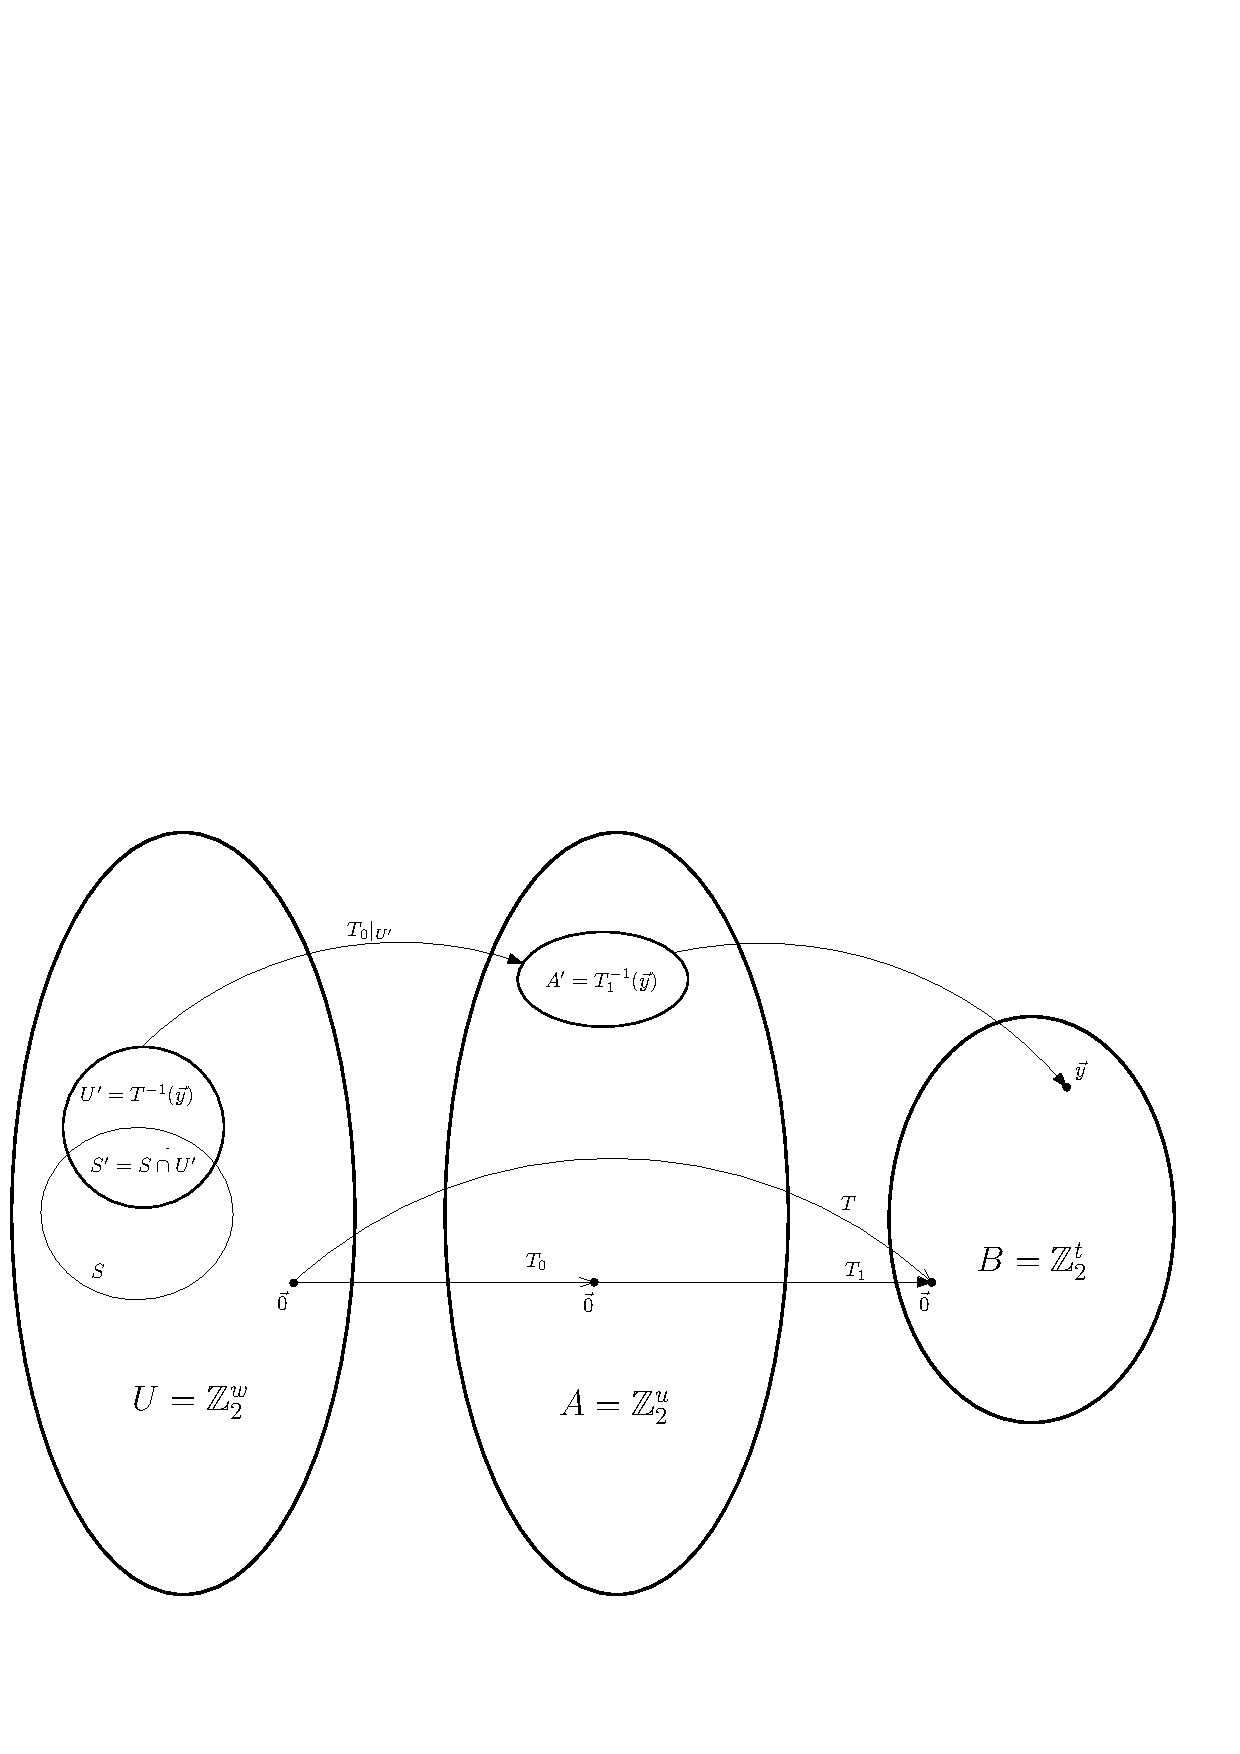
\includegraphics[width=0.9\textwidth]{images/elpsl_proof}
  \caption{Image depicting the situation in the proof.}
\end{figure}

\end{proof}

\begin{corollary}
\label{corollary-prob-e2-e1}
Let $U = \vecspace{w}$, $A = \vecspace{u}$ and $B = \vecspace{t}$. Let $T_0: U \rightarrow A$ and $T_1: A \rightarrow B$ be random uniformly chosen linear transformations where $T_1$ is surjective. Then for every $0 < \epsilon < 1$ there is a constant $c_{\epsilon} > 0$ such that for every $S \subset U$ denoting the hashed  elements and for every $l \in \mathbb{N}$, $l \geq c_{\epsilon}{\frac{|A|}{|B|}}\log\frac{|A|}{|B|}$ for the probability of event $E_1$ we have
\[
	\Prob{E_1(S, T, l)} \leq \frac{1}{1 - \epsilon} \Prob{E_2(S, T_0, T_1)} \text{.}
\]
\end{corollary}
\begin{proof}
The proof is a straightforward use of the previous remark and definition of conditional probability.
\[
	\frac{\Prob{E_2, E_1}}{\Prob{E_1}} = \Prob{E_2 | E_1} \geq 1 - \epsilon
\]

Using the fact $\Prob{E_2} \geq \Prob{E_2, E_1}$ we conclude:
\[
	\Prob{E_1} \leq \frac{1}{1 - \epsilon}\Prob{E_2, E_1} \leq \frac{1}{1 - \epsilon}\Prob{E_2} \text{.}
\]
\end{proof}

The probability bound of existence of a long chain is estimated by the following theorem.
\begin{remark}
\label{remark-probability-long-chain}
Let $U = \vecspace{w}$, $B = \vecspace{t}$ be vector spaces representing the domain ($U$) and the hash table ($B$). Let $T: U \rightarrow B$ be random uniformly chosen linear map and $m = 2 ^ t = |B|$. For every $0 < \epsilon < 1$ and for every $r > 4$ when hashing $S \subset U$, $|S| \leq t 2 ^ t$ following estimate on the length of the longest chain holds.
\[
	\Prob{\lpsl > 4 c_\epsilon r \log m \log \log m} \leq \frac{1}{1 - \epsilon} \left(\frac{r}{\log r}\right)^{-\log \left(\frac{r}{\log r}\right) - \log \log \left(\frac{r}{\log r}\right)} \text{.}
\]
\end{remark}
\begin{proof}
Proof of this remark is a straightforward use of previous remarks, we only have to choose the values of their parameters. As mentioned before we create the factorisation space $A = \vecspace{u}$. By validity of model \ref{remark-model-uniform-linear-map-selection-affine} uniform and independent choice of two random linear transformations $T_0: U \rightarrow A$ and surjective $T_1: A \rightarrow B$ corresponds to the uniform choice $T: U \rightarrow B$ such that $T = T_1 \circ T_0$.

Since $|S| \leq t 2 ^ t$ we have also that $|S| \leq n \log n$. Our choice of $u$ must confirm to $|A| \geq |B|$ since we need a surjective function $T_1$. The choices also satisfy assumptions of the remark \ref{remark-e2-probability} and corollary \ref{corollary-prob-e2-e1}.
\[
\begin{split}
	u & = \left\lfloor \log m + \log \log m + \log r - \log \log r + 1 \right\rfloor \\
	l & = 4c_{\epsilon}r\log m \log \log m \\
\end{split}
\]

Since $r > 4$ we have that $\frac{r}{\log r} > 1$:
\[
	2 ^ u \geq \frac{rm \log m}{\log r} > m \log m \geq 2 ^ t = |B| \text{.}
\]

Hence the condition $d = \frac{|A|}{|S|} > 1$ of remark \ref{remark-e2-probability} is satisfied because
\[
	d = \frac{|A|}{|S|} = \frac{2^u}{m \log m} \geq \frac{m \log m}{m \log m}\frac{r}{\log r} = \frac{r}{\log r} > 1 \text{.}
\]

Following inequality helps us to prove the assumption $l \geq c_\epsilon \frac{|A|}{|B|} \log \frac{|A|}{|B|}$ of the corollary \ref{corollary-prob-e2-e1}.
\[
	\frac{2^u}{m} \leq \frac{2 ^{\log m + \log \log m + \log r - \log \log r + 1}}{m} = \frac{2 r\log m}{\log r}
\]

Because $\log \left(\frac{2 r\log m}{\log r}\right) \leq 2 \log \log m \log r$ the assumption holds:
\[
\begin{split}
c_{\epsilon}\frac{2^u}{m}\log\left(\frac{2^u}{m}\right)
	& \leq 2 c_{\epsilon} \log m \frac{r}{\log r} \log \left(\frac{2 r\log m}{\log r}\right) \\
	& \leq 4 c_{\epsilon} \log m \frac{r}{\log r} \log \log m \log r \\
	& = 4 c_{\epsilon} r \log m \log \log m \\
	& = l \text{.}
\end{split}
\]

Now using remark \ref{remark-e2-probability} and corollary \ref{corollary-prob-e2-e1} we obtain:
\[
\begin{split}
\Prob{E_1}
	& \leq \frac{1}{1 - \epsilon} \Prob{E_2} \\
	& \leq \frac{1}{1 - \epsilon} d ^ {-\log d - \log \log d} \\ 
	& \leq \frac{1}{1 - \epsilon} \left(\frac{r}{\log r}\right)^{-\log \left(\frac{r}{\log r}\right) - \log \log \left(\frac{r}{\log r}\right)} \text{.}
\end{split}
\]

The event $E_1$ denotes the existence of a chain of size at least $l$ elements. A chain longer than $l$ in a hash table exists if and only if the longest chain is longer than $l$, $\lpsl > l \Leftrightarrow E_1(S, T, l)$. This proof completed by writing down the facts observed so far.

\[
\begin{split}
\Prob{\lpsl > l} 
	& = \Prob{\lpsl > 4c_{\epsilon} r \log m \log \log m} \\
	& = \Prob{E_1(S, T, 4c_{\epsilon} r \log m \log \log m)} \\
	& \leq \frac{1}{1 - \epsilon} \left(\frac{r}{\log r}\right)^{-\log \left(\frac{r}{\log r}\right) - \log \log \left(\frac{r}{\log r}\right)} \\
\end{split}
\]
\end{proof}

Previous claim is very convenient in order to successfully prove theorem \ref{theorem-n-logn-to-n}. For every fixed $0 < \epsilon < 1$ set $K_\epsilon = 4 c_\epsilon \log m \log \log m$.
\[
\begin{split}
\Expect{\lpsl}
	& = \int\limits_0^{\infty} \Prob{\lpsl > r} dr \\
	& \leq 4K_\epsilon + \int\limits_{4K_\epsilon}^\infty \Prob{\lpsl > r} dr \\
	& = 4K_\epsilon + K_\epsilon \int\limits_4^\infty \Prob{\lpsl > rK_\epsilon} dr \\
	& \leq 4K_\epsilon + K_\epsilon \int\limits_4^\infty \frac{1}{1 - \epsilon} \left(\frac{r}{\log r}\right)^{-\log \left(\frac{r}{\log r}\right) - \log \log \left(\frac{r}{\log r}\right)} dr \\
	& = K_\epsilon(4 + I_\epsilon) = O(K_\epsilon) = O(\log m \log \log m)
\end{split}
\]

We substituted $I_\epsilon$ for
\[
I_\epsilon = \int\limits_4^\infty \frac{1}{1 - \epsilon} \left(\frac{r}{\log r}\right)^{-\log \left(\frac{r}{\log r}\right) - \log \log \left(\frac{r}{\log r}\right)} dr \text{.}
\]
The fact that this integral is convergent for every $0 < \epsilon < 1$ is shown later.

The proof of the theorem \ref{theorem-n-logn-to-n} is completed even in more general form. We made no special assumptions on the size of the hashed set $S$ except $|S| \leq |B| \log |B|$. \qed

\mbox{\qedhere}

Multiplicative constant $4 c_\epsilon(4 + I_\epsilon)$ plays an important role for a practical use of this result. In our proofs performed so far we neglected its estimation. We only obtained a good asymptotic result that is negated by the constant's great value. For example when choosing $\epsilon$ equal to $\frac{1}{2}$ only constant $c_\epsilon$ equals $4 ^ {17}$ by usage of the original estimate. Our next goal is to show a better constant's estimate, explore the dependency of the longest chain on load factor of the hash table and find an even better constant when using load factors lower than one.
\end{section}

\begin{section}{Hashing a linear amount of elements with respect to the table's size}
Usage of the hash table with load factors lower than one brings us even lower expected lengths of the longest chains. This situation lowers the multiplicative constant and this is the reason why we examine this case. We already showed if a super-linear amount of elements is hashed then we can expect reasonable worst case behaviour. However the most important is the real expected size of a bucket. Upper bound on the expected operation's running time is equal to $1 + c \alpha$ in every model of universal hashing. So using load factors lower than one has significant impact on the expected case. We must examine a scheme of hashing $n = \alpha m$ elements into a hash table of size $m$. 

\begin{theorem}
\label{theorem-n-to-n}
Assume that the table's load factor $\alpha$ is bounded in $\left[0.5, 1\right]$. Then whenever hashing $\alpha m$ elements into a table of size $m$ the expected length of the longest chain is bounded by $O(\alpha \log m \log \log m)$.
\end{theorem}
\begin{proof}

In the case of hashing $m \log m$ elements we prepared some useful and remarks in advance and then finished main proof. We have to modify them, especially the choices for the size of the factor space differ. Apparently we must lower the value of a chain length when we get a convenient probability estimate proportionally to $\alpha_f$. 

\begin{remark}
Suppose a model of hashing domain $U = \vecspace{w}$ to a hash table $B = \vecspace{t}$ and define $m = |B|$. Assume we use $LT(U, B)$ as universal class and let $T \in LT(U, B)$ be a random uniformly chosen linear map used as a hash function. Moreover let $S \subset U$ be hashed set such that $|S| = \alpha m$ for load factor $0.5 \leq \alpha \leq 1$. Then for every $0 < \epsilon < 1$ there and $r > 4$,  probability of existence of a long chain is bounded as:
\[
\Prob{\lpsl > 4 c_\epsilon \alpha r \log m \log \log m} \leq \frac{1}{1 - \epsilon} \left(\frac{r}{\log r}\right)^{-\log \left(\frac{r}{\log r}\right) - \log \log \left(\frac{r}{\log r}\right)} \text{.}
\]
\end{remark}
\begin{proof}
We just show how the choices have to be made to prove the remark. We use the same approach and follow the proof of remark \ref{remark-probability-long-chain}. Just remember that we factored through the vector space $A = \vecspace{u}$ and the choice of its dimension has been made. We used a uniform model of selection of two linear functions $T_0: U \rightarrow A$ and surjective $T_1: A \rightarrow B$ such that $T = T_1 \circ T_0$. This gave us uniform choice of $T$.

\[
\begin{split}
	u & = \left\lfloor \log m + \log \log m + \log r - \log \log r + \log \alpha + 1 \right\rfloor \\
	l & = 4 c_\epsilon \alpha r \log m \log \log m \\
	d & = \frac{|A|}{\alpha m \log m}
\end{split}
\]

In order to ensure existence of surjective mapping $T_1$ we have to verify that $|A| \geq |B|$.
\[
	|A| = 2 ^ u \geq \frac{\alpha m \log m r}{\log r} \geq m \log m \geq |B|
\]

We slightly changed the choice of variable $d$. In the original remark \ref{remark-e2-probability} we defined $d$ as $\frac{|A|}{|S|}$ but in its proof three inequalities concerning $d$ were needed.
\[
\begin{split}
	d & > 1 \\
	\mu & = 1 - \frac{|A - T_0(S)|}{|A|} \leq \frac{1}{d} < 1 \\
	\log d & \geq u - t - \log t \\
\end{split}
\]

To keep remark \ref{remark-e2-probability} in validity we have to verify each of them. For the first one we can use just observed fact $|A| > |B|$.
\[
	d = \frac{|A|}{\alpha m \log m} \geq \frac{m \log m}{\alpha m \log m} = \frac{1}{\alpha} \geq 1
\]

The second one.
\[
	\mu = 1 - \frac{|A - T_0(S)|}{|A|} = \frac{|T_0(S)|}{|A|} \leq \frac{|S|}{|A|} = \frac{\alpha |B|}{|A|} \leq \frac{\alpha m \log m}{|A|} = \frac{1}{d} < 1
\]

And the third one follows. Just remember the bound on $\alpha$, $\alpha \in \left[0.5, 1\right]$ and this implies that $\log \alpha \leq 0$.
\[
	\log d = u - \log \alpha - \log |B| - \log \log |B| = u - t - \log t - \log \alpha \geq u - t - \log t
\]

The assumptions of modified remark \ref{remark-e2-probability} are met. For using the other remark, \ref{remark-prob-l-length-chain}, the value of the variable $l$ has to be large enough:
\[
\begin{split}
c_{\epsilon} \frac{|A|}{|B|} \log \left(\frac{|A|}{|B|}\right) 
	& = c_{\epsilon} \frac{2^u}{m} \log \left(\frac{2^u}{m}\right) \\
	& < 2 c_{\epsilon} \alpha \log m \left( \frac{r}{\log r} \right) \left(2 \log \log m \log r \right) \\
	& \leq 4 c_{\epsilon} \alpha r \log m \log \log m \\
	& = l
\end{split}
\]

The conditions of both remarks \ref{remark-e2-probability} and \ref{remark-prob-l-length-chain} are satisfied. We can carry on identically as in the case without the load factor. In order to express probability density function of the variable $\lpsl$ we have to estimate $\Prob{E2(S, T_0, T_1)|E1(S, T, l)}$. Now use theorem \ref{theorem-set-onto-by-linear-transform} for sets $U' = T^{-1}(\vec{y})$, $A' = T_1^{-1}(\vec{y})$ and restricted $T_0|_U'$ as in the original proof. Vector $\vec{y}$ is taken from appearance of the event $E_2(S, T, l)$ and define $S' = U' \cup S$.
\[
	\Prob{T_0|_{U'}(S') = A' | E1} \geq 1 - \epsilon
\]

As in the previous case whenever $T_0|_{U'}(S') = A'$ event $E2$ appears as well and we conclude.

\[
\begin{split}
\Prob{E1} 
	& \leq \frac{1}{\Prob{E2|E1}}{\Prob{E2}} \\
	& \leq \frac{1}{1 - \epsilon} d ^ {-\log d - \log \log d} \\
	& = \frac{1}{1 - \epsilon} \left(\frac{r}{\log r}\right)^{-\log \left(\frac{r}{\log r}\right) - \log \log \left(\frac{r}{\log r}\right)} \text{.}
\end{split}
\]

For the last inequality we used the fact $d \geq \frac{r}{\log r} > 1$.
\[
	d = \frac{|A|}{\alpha m \log m} \geq \frac{2 \alpha m \log m}{\alpha m \log m} \frac{r}{\log r} \geq \frac{r}{\log r}
\]

Now we have since $\frac{1}{d} \leq \frac{\log r}{r} < 1$:
\[
\begin{split}
d ^ {-\log d - \log \log d} 
	& = \left(\frac{1}{d}\right) ^ {\log d + \log \log d} \\
	& \leq \left(\frac{1}{d}\right) ^ {\log \left(\frac{r}{\log r}\right) + \log \log
 \left(\frac{r}{\log r}\right)} \\
	& \leq \left(\frac{\log r}{r}\right) ^ {\log \left(\frac{r}{\log r}\right) + \log \log
 \left(\frac{r}{\log r}\right)} \\
	& = \left(\frac{r}{\log r}\right)^{-\log \left(\frac{r}{\log r}\right) - \log \log \left(\frac{r}{\log r}\right)} \text{.}
\end{split}
\]
\end{proof}

In order to achieve the desired expected longest chain length we perform similar computation as in the original theorem. Now we set $K = 4 \alpha c_\epsilon \log m \log \log m$.
\[
\begin{split}
\Expect{\lpsl}
	& = \int\limits_0^\infty \Prob{\lpsl > r} dr \\
	& \leq 4K + \int\limits_{4K}^\infty \Prob{\lpsl > r} dr \\
	& = 4K + K\int\limits_4^\infty \Prob{\lpsl > rK} dr \\
	& \leq K(4 + I_\epsilon) = O(K) = O(\alpha \log m \log \log m)
\end{split}
\]
\end{proof}
\end{section}
